
\section{Personalized Medicine}

A medium-term goal of medicine is ``personalized medicine\index{personalized medicine}'',
whose goal is to provide custom-tailored health care on an individual
basis. For example, a standard treatment for breast cancer is chemotherapy,
but not all patients profit from this treatment. The event that a
patient has no sign of breast cancer after reductive surgery followed
by chemotherapy is called \emph{pathologic complete response}\index{pathologic complete response}\index{pCR},
and the opposite event that the patient still has cancerous tissue
after this procedure is called \emph{residual disease}\index{residual disease}\index{RD}.

Suppose there were a predictor that could tell the physicist how likely
a patient is to benefit from chemotherapy. If the prediction for a
certain patient was such that complete response to chemotherapy was
unlikely, chemotherapy could be replaced by another therapy.

The goal of this work is to contribute to such a predictor. The input
to the predictor is the molecular expression data, i.e. measures of
the number of RNA copies of specific genes present in the cancer tissue.
These gene expression measurements are ususally measured using microarrays
or next generation sequencing. An artificial neural network then processes
this data. The prediction is output by the network in the form of
a number between 0 and 1. Here, 0 means the patient is predicted with
absolute certainty to have residual disease, 1 means the patient is
predicted with absolute certainty to have pathologic complete response,
and a number in-between is interpreted as the probability for pathologic
complete response.

The study of neural networks in biology prompted the development of
artificial neural networks as models of biological neural networks.
After an introduction to biological and artificial neural networks
we will give an overview of the relevant topics of machine learning
and then introduce the own work done in this manuscript.

\section{Biological and Artificial Neural Networks}

Artificial neural networks\index{artificial neural networks} are
mathematical constructs, designed to imitate the signal processing
capabilities of real neurons, found in nearly all animals. Neurons
can be connected to form complex neural networks. Like their biological
counterparts, artificial neural networks consist of simpler building
blocks, the neurons.

\subsection{Neurons As Basic Signal Processing Units}

The biological neurons are defined (according to the neuron doctrine
\cite{BullockDouglas2005}) as the smallest units whose state change
may be called signal processing, so they are the basic signal processing
units. They have multiple inputs at dendrites, and multiple outputs
at axon terminals \cite{ByrneDafny1997}. Figure \ref{fig:Schematic-image-of-biological-neurons}
gives a schematic overview of these elements.

\begin{figure}
\begin{centering}
\includegraphics[width=0.8\columnwidth]{images/neurons}
\par\end{centering}
\caption[Schematic image of three biological neurons.]{\label{fig:Schematic-image-of-biological-neurons}Schematic image
of three biological neurons. A: neuron body B: nucleus C: dendrite
D: synapse E: axon projecting from a distant neuron.}
\end{figure}

In most real neurons, the signal transmission and processing is facilitated
by alternating small electric (action) potentials (along the axons)
and chemical transmissions (at chemical synapses between axon and
dendrite). The electric potential is transmitted along the dendrites
of a neuron, and flows to the axon of the neuron, where it can lead
to the release of neurotransmitters stored in the axon terminals into
the synaptic cleft. The released neurotransmitters are detected by
receptors and cause ion channels in the adjacent dendrites of other
neurons to open, which changes their membrane potential. See figure
\ref{fig:Schema-of-chemical-synapse} for a depiction of axon, synaptic
cleft, and dendrite.

\begin{figure}[t]
\begin{centering}
\includegraphics[width=0.8\columnwidth]{images/synapse}
\par\end{centering}
\caption[Schema of a chemical synapse.]{\label{fig:Schema-of-chemical-synapse}Schema of a chemical synapse.
The signal is transmitted from the axon terminal (left) to the dendrite
(right). Grey: membranes of neurons. Green and blue: ion transporters
maintain intracellular ion concentrations. Red: neurotransmitter is
stored inside the cell in vesicles and emitted into the synaptic cleft
upon an electric potential arriving at the axon terminal. Purple:
receptors signal to the inside of the cell the absence or presence
of neurotransmitter on the outside of the cell.}
\end{figure}

\subsubsection{Action Potentials, Their Propagation, and Chemical Synapses }

The action potentials are realized by cells in the form of different
ion concentrations inside and outside the cell. These ion gradients
are maintained in the resting state by the $Na^{+}/K^{+}$-ATPases
that pump 3 $Na^{+}$ ions out of and 2 $K^{+}$ ions into the cell
for every ATP molecule \cite{LodishZipursky2000}. Because ions are
charged, there is an electric potential between the outside and inside
of the cell. The resting potential is between $-80$mV and $-40$mV,
depending on the type of neuron. The electric potential becoming more
positive is called depolarization, and the opposite hyperpolarization.

The propagation of the action potentials along dendrites is realized
by the opening and closing of ion channels. Once depolarization of
an adjacent region of a neuron causes the electric potential between
the inside and outside of a $Na^{+}$ ion channel to reach a critical
value, the ion channel opens, causing further depolarization in adjacent
regions of the neuron. This positive feedback loop continues until
all $Na^{+}$ channels are open. At the peak of depolarization, $K^{+}$
ion channels open, causing hyperpolarization, and the potential returns
to the resting  potential. This makes the action potential travel
along the neuron. Once it has reached an axon terminal, it causes
neurotransmitter release.

Neurotransmitters binding to receptors present on the outside of
the neuron's membrane cause ion channels to open, and the ions flow
into or out of the cell to achieve equilibrium of ion concentration.
The type of ion channel being opened upon binding of a neurotransmitter
can cause either depolarization or hyperpolarization of the dendrite,
depending on the charge of the ion, and whether the resting concentration
of the ion is higher intracellular or extracellular. If a critical
threshold of depolarization is reached, the $Na^{+}$ ion channels
will open, and an action potential ``spike'' is generated as described
above.

\subsubsection{Encoding of Information in Action Potentials}

The presence of a critical threshold suggests that it is not the ``analog''
electric potential, but the ``digital'' spike that carries the information
from one neuron to the next. For example, the strength muscles are
innervated with, is encoded in the number of action potentials per
time delivered by the muscle neuron to the muscle fiber. However,
some neurons involved in perception directly transmit information
in the fluctuations of neurotransmitter released. This analog mode
of transmission allows more information to be transmitted per time.
Sub\-threshold emission of neurotransmitter also seems to modulate
subsequent action potentials, allowing for a mixture of analog and
digital information transmission \cite{DebanneRama2013}. 

Examples for neural networks that have been partly decoded are the
eye (visual system) and the nose (olfactory system).

\subsection{Examples of Biological Neural Networks}

\subsubsection{The Eye, a Visual System}

In the eye, specialized cells called rods and cones detect light\cite{Biochemistry2002,Kolb2003}.
Rods are more sensitive to dim light, while the three types of cones
react to bright light only but can differentiate between colors. Both
rods and cones release the neurotransmitter glutamate continuously
into the synaptic cleft, but when hit by light, suspend this emission
for the duration of the light. This is implemented by the cell by
a long pathway.

Specifically, light elicits a transformation of cis-rhodopsin to trans-rhodopsin,
which presents on its surface a G protein binding site. The G protein
transducin binds to the activated rhodopsin, and in this process GDP
acquires a phosphate group to form GTP. The $\alpha$-subunit of transducin
activates a cGMP phosphodiesterase, which in turn hydrolyzes cGMP
to GMP. The reduction in the concentration of cGMP causes cGMP-gated
ion channels to close. This in turn hyperpolarizes the photosensitive
cell, causing glutamate to be released into the synaptic cleft at
a slower rate. This long pathway between cis-rhodopsin and glutamate
release inhibition facilitates an amplification of the signal at every
step, which allows rod cells to signal a spike in response to it being
hit by a single photon.

The area that elicits a response in the cell upon being illuminated
is called the \emph{receptive field}\index{receptive field}, and
is just as large as the top of the photoreceptor for rods and cones.
The released glutamate binds to receptors present on the outside of
bipolar cells, and, depending on the type of bipolar cell, cause either
an action potential to be generated when the photoreceptor is lit
and the surrounding area is dark (\emph{ON }bipolar cell), or when
the photoreceptor is dark against a bright background (\emph{OFF }bipolar
cell). Another type of cell, the horizontal cell integrates signals
from surrounding cone cells, and feed their signal back to the cones,
or directly to bipolar cells. This enhances contrast. The signal from
several bipolar cells is fed into a ganglion cell, which therefore
has a larger receptive field than its connected bipolar cells. ON
bipolar cells only excite ON ganglion cells, and OFF bipolar cells
excite only OFF ganglion cells. Finally, in primates, there are more
than a million nerve fibers from ganglion cells to the visual cortex
of the brain. Altogether, the basic cell types are, depending on the
species, 1 to 4 types of horizontal cells, 11 types of bipolar cells,
22 to 30 types of amacrine cells, and 20 types of ganglion cells.
Among those cell types' known functions are integration of a large
number of rods to provide sight in little light, brightness-dependent
size regulation of the receptive field of amacrine cells, and an additional
photoreceptor distinct from rods and cones\cite{Kolb2003}.


\subsubsection{Odor Sensing in the Olfactory System}

The olfactory system of mammals and insects contains neurons that
detect odor molecules, called glomeruli\cite{ZhangSharpee2016}. In
humans, there are about $500$ different types of glomeruli {[}1{]},
but it is hypothesized that a human can perceive around $10,000$
different odors. Each ``atomic'' odor consisting of a few ($<100$)
molecular species excites one or more glomeruli, and the compression
requires each glomerulus to signal the presence of one or more than
one odor. The excitation pattern of multiple glomeruli must be resolved
in the olfactory neuronal system so that a low-dimensional vector
of ($\approx500$) glomeruli activations is decompressed to a high-dimensional
representation of ($\approx10,000$) odors in the brain.

Each glomerulus is connected to one or more Kenyon Cells in insects.
It is assumed that the activation of a Kenyon cell signals to the
insect nervous system the presence of one specific odor. (In the mammalian
brain, a single odor is represented by neurons in the olfactory cortex.)
Experiments show that the circuit connecting glomeruli to Kenyon cells
is feed-forward\index{feed-forward neural network} only, i.e. without
recurrent connections (loops). The structure of a feed-forward compressed
sensing circuitry is of interest, because standard compressed sensing
circuits are recurrent dynamic systems that converge to one of their
attractor states. In addition to quick decoding of odors, experimental
evidence shows that the biological compressed sensing circuitry is
robust to noise, i.e. to spurious neuronal spikes in glomeruli, or
noise due to experimental inhibition\footnote{Also experimental modifications of glomeruli have been made so that
half of all glomeruli always express only one type of receptor.} of glomeruli.

The theoretical work of \cite{ZhangSharpee2016} proposed that a feed-forward
architecture could facilitate odor decoding simply by implementing
a logical AND. They suggest that in the neuronal AND-circuit a specific
odor's Kenyon cell is activated when at least (for example) $80\%$
of the glomeruli with receptors to this odor are active. On a cellular
level, this could be realized by connecting the glomeruli associated
with an odor with the odor's Kenyon cell, and a threshold at the Kenyon
cell's input.

A prediction of \cite{ZhangSharpee2016} is that the number of glomeruli
activated by a single odor should be close to the number of glomeruli
that are connected to a Kenyon cell. They postulated further that
the validity of their feed-forward model can be tested by measuring
the odor sparseness\footnote{Odor sparseness is the average number of different molecular species
in an odor.} in the environment of an animal species and comparing it to its average
number of connections from glomeruli to Kenyon cells.

For example, in \emph{Drosophila}, about $9\%$ of the glomeruli are
excited by an odorant, and the connectivity rate between glomeruli
and Kenyon Cells is between $6.5\%$ and $12.5\%$. In the locust,
a projection neuron (the equivalent to a glomerulus) is activated
by half of the odorants and the connectivity rate is about $50\%$.
This is in agreement with the proposed model.

The model also predicts that species with sparse connectivity have
better odor perception of complex odor mixtures. On the other hand,
species with dense connectivity should have better olfactory performance
in detecting simple odor mixtures.

\subsection{Artificial Neurons as Simple Models of Biological Neurons\label{subsec:Artificial-Neurons-as-Simple-Models-of-Biological-Neurons}}

The machinery facilitating propagation and transmission of information
in and between biological neurons is highly simplified in artificial
neurons\index{artificial neuron signal processing}. Signal processing
of a real neuron is modelled in an artificial neuron as a mathematical
function that has multiple input variables, computes a value according
to the function formula and its parameters and outputs its computed
value to multiple neurons, which use it as an input variable. Herein,
the processes of neurotransmitter release, de- and hyperpolarization,
and propagation of the action potential are abstracted away into discrete
time steps.

Each artificial neuron's function is evaluated once per time step.
Often, the \emph{sigmoid}\index{sigmoid function}\emph{ }function
is used to describe the output of an artificial neuron, the so-called
\emph{activation}\index{activation of an artificial neuron}

\begin{equation}
o_{i}=\sigma(v_{i})=\frac{1}{1+\exp(-v_{i})},\label{eq:sigmoid-function}
\end{equation}
where $v_{i}\in\mathbb{R}$ is the accumulated input to neuron $i$,
and $o_{i}\in[0;1]$ is the activation of neuron $i$. See the left
panel of figure \ref{fig:sigmoid-function} for a plot of the sigmoid
function.
\begin{figure}
\begin{centering}
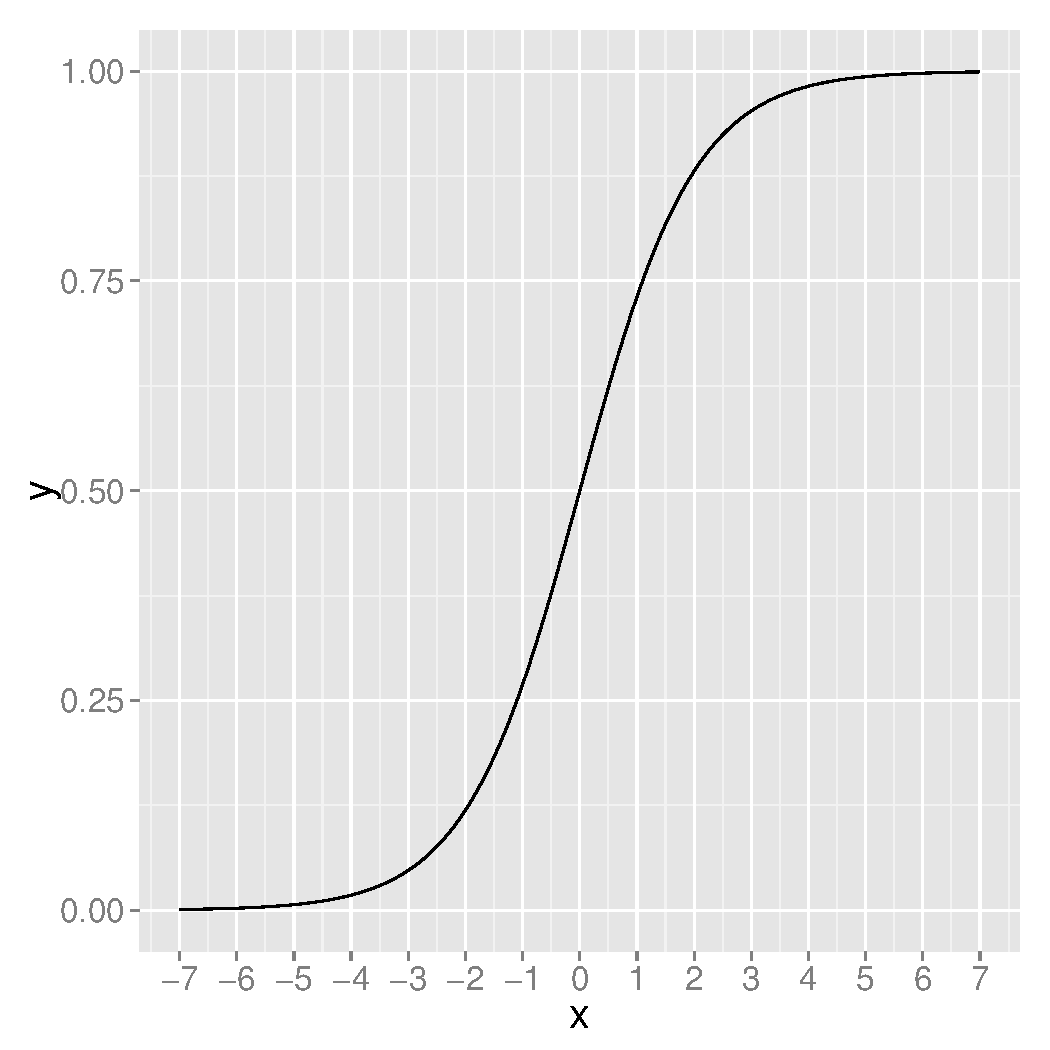
\includegraphics[width=0.45\columnwidth]{images/plot-sigmoid}\hfill{}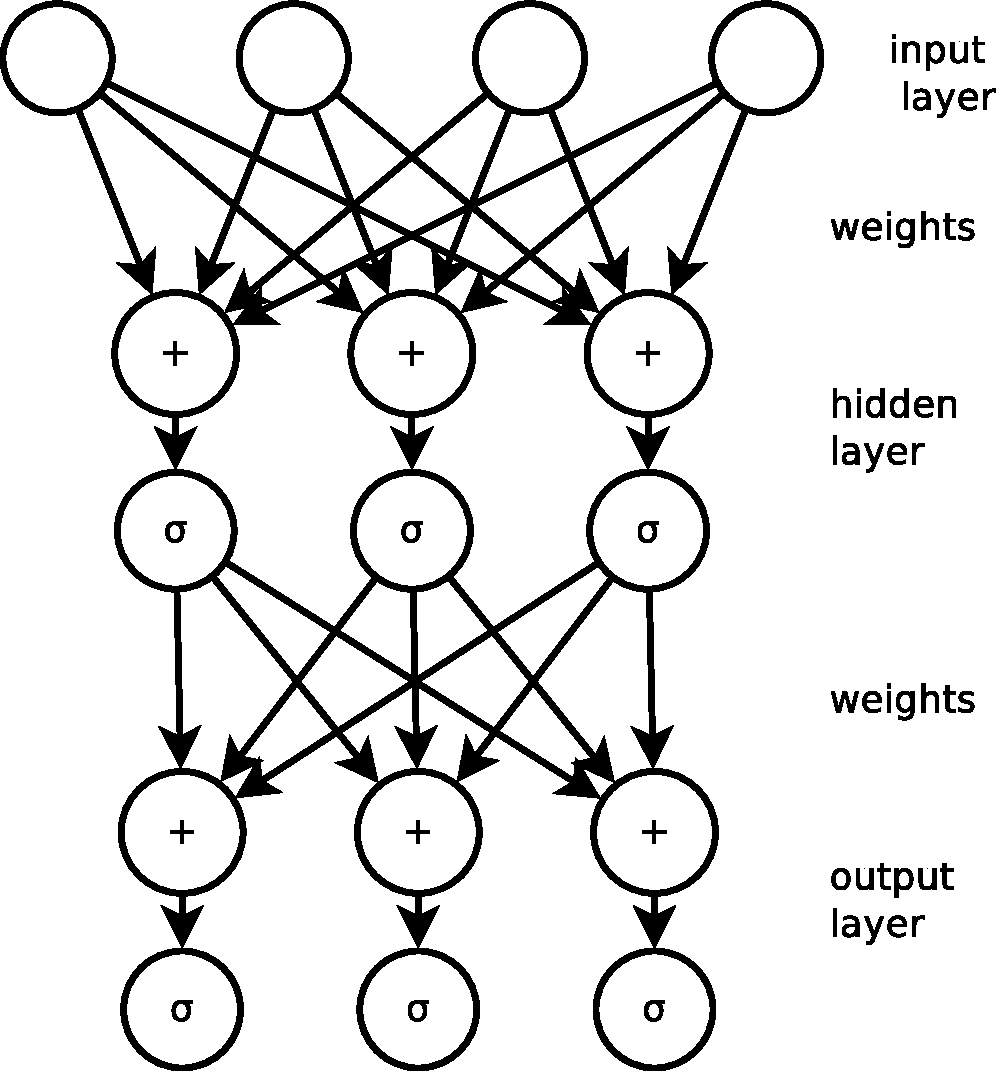
\includegraphics[width=0.45\columnwidth]{images/neuronal-network-example}
\par\end{centering}
\caption{\label{fig:sigmoid-function}Left: The sigmoid function $\sigma$.
Right: Schema of the computational steps in an artificial neural feed-forward
network\index{feed-forward neural network} from input layer to output
layer. The ``+'' nodes accumulate their input values, and the ``$\sigma$''
nodes compute the output of a neuron, to be used as input for the
next layer.}
\end{figure}

The effect of an incoming axon onto a neuron, that is, the different
types of receptors that can be present on the outside of a real dendrite,
and the effected de- or hyperpolarization of the dendrite are abstracted
away by using real-numbered weights. Weights are parameters to the
mathematical function describing the conversion of outputs of neurons
to the single input of the next connected neuron. Usually the input
$v_{i}$ of neuron $i$ is computed from the outputs of its connected
neurons $\mathbf{c_{i}}$ as in
\begin{equation}
v_{i}=b_{i}+\sum_{j\in\mathbf{c_{i}}}o_{j}w_{ij},\label{eq:input-to-a-neuron}
\end{equation}
where $b_{i}\in\mbox{\ensuremath{\mathbb{R}}}$ is the so-called \emph{bias}\index{bias of an artificial neuron}\emph{
}of neuron $i$, $\mathbf{c_{i}}$ is the vector of indices of its
in-going connected neurons, $o_{j}\in\mathbb{R}$ is the activation
of the connected neuron $j$, and $w_{ij}\in\mathbb{R}$ is the weight
of the connection going out of neuron $j$ and into neuron $i$.

In an neural network the neurons are often arranged in layers. See
the right panel of figure \ref{fig:sigmoid-function} for an example
of the structure of an artificial neural network.

\subsection{Learning in Biological Neural Networks}

Nervous systems do not only process signals, but they also learn,
that means that they adapt their signal processing over time. One
reason for this is an organism's need for a change in behavior, as
response to a changing environment.

In biological neuronal systems, this is possible by altering existing
synapses (for example by exchanging the receptors on the surface of
dendrites), or by creating and abandoning existing synapses (i.e.
connecting the axon terminals of a neuron to different neurons). There
are several known cellular mechanisms for that, among them LTP, LTD,
and PTP\cite{BermudezFederico2007}. Strengthening of the synaptic
link (that occurs within minutes and remains after hours and up to
weeks in the hippocampus of mammals) is called long-term potentiation
(LTP), while its weakening is called long-term depression (LTD). LTP
is induced by associativity of connected neurons, that means, when
a neuron contributes to the depolarization in a directly connected
neuron, the efficiency of that connection will be strengthened. The
molecular mechanisms responsible for this phenomenon are not yet completely
understood. It is known that they differ between brain regions, and
also between types of synapses in the same brain region. The cellular
mechanisms controlling these processes, and their interplay in larger
neuron ensembles are a field of active research \cite{BermudezFederico2007}.

An unproven hypothesis is that learning is local\index{locality of Hebbian learning rule},
which means that changes at a synapse only depend on the directly
connected neurons, but not on other distantly-connected neurons. This
type of local learning is called \emph{Hebbian learning}\index{Hebbian learning}.

The learning in biological neuronal systems happens seemingly automatically,
for example, migratory birds learn and remember travel paths around
the globe, without an apparent teacher. Ultimately the goals of learning
are determined by an interplay of evolution and the environment. 

\subsection{Back-propagation for Training Artificial Neural Networks\label{subsec:Back-propagation}}

The nearest analog to learning in biological neural networks is \emph{training
}artificial neural networks\index{training of artificial neural networks}.
Here, the goal is explicitly set by humans by providing training data
sets. One training sample consists of a vector of real numbers called
\emph{input patterns}\index{input pattern} and a corresponding vector
of real numbers of desired \emph{output patterns}\index{output pattern},
also called \emph{labels}\index{label}. For every input pattern in
the training data set an output pattern is defined that the learner
should compute from the input pattern. Learning is hereby facilitated
by changing the parameters of the artificial neural network.

Back-propagation is a supervised training procedure for artificial
neural networks \cite{RumelhartWilliams1988}. It learns from labeled
training samples. The parameters of the network, the weights and biases,
are adapted using \emph{gradient descent}\index{gradient descent}.
The basic idea is to set the neurons in the input layer to the input
pattern, compute the activations of neurons in the network, compute
the total error observed in the output layer using the difference
between actual and desired output, then determine how much each neuron
was ``responsible'' for the total error in the network, and finally
use it to adapt the weights and biases. This procedure is then repeated
until the network is fully trained.

Let the supervised training patterns be indexed by $p$, $x_{i,p}$
the activation of a neuron $i$ in the input layer for training pattern
$p$, and $y_{k,p}$ the desired activation of neuron $k$ in the
output layer for this training pattern.

\paragraph{Forward Pass}

The supervised training procedure first performs the \emph{forward
pass}\index{forward pass}: it sets activations $o_{i}$ in the input
layer according to the input pattern $x_{i,p}$ to be learned, computes
the activations $o_{j}$ of the hidden layers and the output layer
$o_{k}$.

(In the following, index $k$ is used for a neuron in the output layer,
and indices $j$ and $i$ for a neuron in a hidden layer or the output
layer. If the network has only one hidden layer, then index $i$ refers
to a neuron in the input layer.)

Each input neuron's output $o_{i}$ is set to a training input: 
\begin{equation}
o_{i}=x_{i,p}.
\end{equation}
The input $v_{j}$ to a hidden or output neuron is computed from the
sum of the connected neurons' outputs in the layer above (see section
\ref{subsec:Artificial-Neurons-as-Simple-Models-of-Biological-Neurons}
):
\begin{equation}
v_{j}=b_{j}+\sum_{i\in\mathbf{c_{j}}}o_{i}w_{ji},
\end{equation}
 where $b_{j}$ is the bias, $o_{i}$ is the output of a neuron in
the layer above, and $w_{ji}$ is the weight of the connection from
neuron $i$ to neuron $j$. The input $v_{j}$ is then scaled by the
sigmoid function to produce a neuron's output $o_{j}$:

\begin{equation}
o_{j}=\sigma(v_{j})=\frac{1}{1+\exp(-v_{j})}.\label{eq:sigmoid-function-2}
\end{equation}

\paragraph{Backward Pass for the Output Layer}

While in the forward pass the information flowed from input to output
layer, in the \emph{backward pass}\index{backward pass}, the information
flows from output to input layer, adjusting the weights and biases
on the way. See figure \ref{fig:Data-flow-in-back-propagation} for
an illustration of the two data flow directions.

\begin{figure}
\begin{centering}
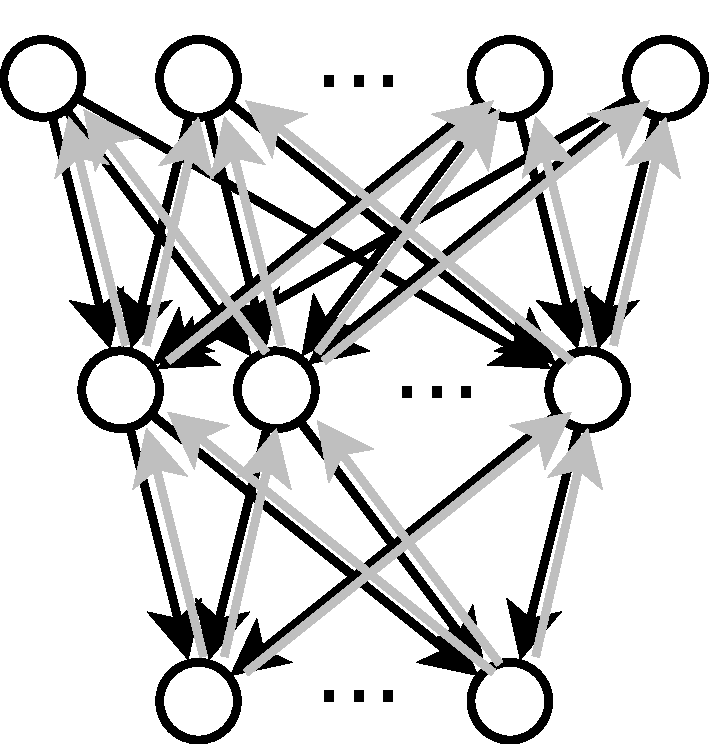
\includegraphics[width=0.34\columnwidth]{images/introduction-backpropagation-data-flow}
\par\end{centering}
\caption[Data flow in training a neural network using back-propagation.]{\label{fig:Data-flow-in-back-propagation}Data flow in training a
neural network with three layers using back-propagation. The input
layer is at the top, the hidden layer in the middle, and the output
layer at the bottom. The black arrows denote information flow during
the forward pass. Each black arrow is associated with a weight from
tail to head. The grey arrows denote information flow during the backward
pass, which propagates errors in the reverse direction.}
\end{figure}
The training procedure computes the total error $E_{total}$ of the
network, which is defined as the squared sum of differences between
actual output $o_{k}$ and desired output $y_{k}$ over all training
patterns:
\begin{eqnarray}
E_{total} & = & \sum_{p}\sum_{k}\frac{1}{2}(o_{k,p}-y_{k,p})^{2}\\
 & = & \sum_{p}E,\nonumber 
\end{eqnarray}
 where $E$ is the error of one training pattern. We further split
$E$ into a sum of errors of individual neurons $E_{k}$: 
\begin{eqnarray}
E & = & \sum_{k}\frac{1}{2}(o_{k}-y_{k})^{2}\\
 & = & \sum_{k}E_{k},\nonumber 
\end{eqnarray}
where $E_{k}=\frac{1}{2}(o_{k}-y_{k})^{2}$. To compute the contribution
of weight $w_{kj}$ to the error, the error $E$ is then differentiated
with respect to a weight $w_{kj}$ for a connection from neuron $j$
in the last hidden layer to neuron $k$ in the output layer: 
\begin{eqnarray}
\frac{\partial E}{\partial w_{kj}} & = & \frac{\partial E}{\partial o_{k}}\cdot\frac{\partial o_{k}}{\partial v_{k}}\cdot\frac{\partial v_{k}}{\partial w_{kj}}\nonumber \\
 & = & \frac{\partial\sum_{k}E_{k}}{\partial o_{k}}\cdot\frac{\partial o_{k}}{\partial v_{k}}\cdot\frac{\partial v_{k}}{\partial w_{kj}}\nonumber \\
 & = & \frac{\partial E_{k}}{\partial o_{k}}\cdot\frac{\partial o_{k}}{\partial v_{k}}\cdot\frac{\partial v_{k}}{\partial w_{kj}}\label{eq:backpropagation-error-wrt-weight-output-layer}\\
 & = & (o_{k}-y_{k})\cdot o_{k}(1-o_{k})\cdot o_{j},\nonumber 
\end{eqnarray}
 which uses that the derivative of the sigmoid function $o_{k}=\frac{1}{1+\exp(-v_{k})}$
is $\frac{\partial o_{k}}{\partial v_{k}}=o_{k}(1-o_{k})$. The derivative
of the error with respect to $b_{k}$ is
\begin{equation}
\frac{\partial E}{\partial b_{k}}=\frac{\partial E}{\partial o_{k}}\cdot\frac{\partial o_{k}}{\partial v_{k}}\cdot\frac{\partial v_{k}}{\partial b_{k}}=(o_{k}-y_{k})\cdot o_{k}(1-o_{k})\cdot1.
\end{equation}

\paragraph{Backward Pass for the Other Layers}

To perform gradient descent, we also need to update the weights and
biases for the remaining connections between hidden layers, and from
the input layer to the first hidden layer. The derivative of the error
with respect to the weight $w_{ji}$ of the connection from neuron
$i$ in a layer to neuron $j$ in the layer below (for example, from
neuron $i$ in the second last hidden layer to neuron $j$ in the
last hidden layer) is
\begin{eqnarray}
\frac{\partial E}{\partial w_{ji}} & = & \frac{\partial E}{\partial o_{j}}\cdot\frac{\partial o_{j}}{\partial v_{j}}\cdot\frac{\partial v_{j}}{\partial w_{ji}}\label{eq:backpropagation-error-wrt-weight-other-layers}\\
 & = & \frac{\partial E}{\partial o_{j}}\cdot o_{j}(1-o_{j})\cdot o_{i},\nonumber 
\end{eqnarray}
 where 
\begin{eqnarray}
\frac{\partial E}{\partial o_{j}} & = & \frac{\partial}{\partial o_{j}}\sum_{k}E_{k}\nonumber \\
 & = & \sum_{k}\frac{\partial}{\partial o_{j}}E_{k}\nonumber \\
 & = & \sum_{k}\frac{\partial E_{k}}{\partial o_{k}}\frac{\partial o_{k}}{\partial v_{k}}\cdot\frac{\partial v_{k}}{\partial o_{j}}\nonumber \\
 & = & \sum_{k}\frac{\partial E_{k}}{\partial o_{k}}\frac{\partial o_{k}}{\partial v_{k}}\cdot w_{kj},\label{eq:backpropagation-error-wrt-output-other-layers}
\end{eqnarray}
and neuron $k$ is in the layer below the layer that neuron $j$ is
in (in our example neuron $k$ is in the output layer). We take the
value for $\frac{\partial E_{k}}{\partial o_{k}}\frac{\partial o_{k}}{\partial v_{k}}$
in equation \ref{eq:backpropagation-error-wrt-output-other-layers}
above from equation \ref{eq:backpropagation-error-wrt-weight-output-layer}
when neuron $k$ is in the output layer or equation \ref{eq:backpropagation-error-wrt-weight-other-layers}
when neuron $k$ is in a hidden layer. (Neuron $k$ is named $j$
in equation \ref{eq:backpropagation-error-wrt-weight-other-layers}.)
In our example (for neuron $j$ in the last hidden layer), we take
$\frac{\partial E_{k}}{\partial o_{k}}\frac{\partial o_{k}}{\partial v_{k}}$
from the output layer: 
\begin{eqnarray}
\frac{\partial E}{\partial o_{j}} & = & \sum_{k}\frac{\partial E_{k}}{\partial o_{k}}\cdot\frac{\partial o_{k}}{\partial v_{k}}\cdot w_{kj}\\
 & = & \sum_{k}(o_{k}-y_{k})\cdot o_{k}(1-o_{k})\cdot w_{kj}.\nonumber 
\end{eqnarray}
Analogously, the derivative of $E$ with respect to $b_{j}$ is 
\begin{eqnarray}
\frac{\partial E}{\partial b_{j}} & = & \frac{\partial E}{\partial o_{k}}\frac{\partial o_{k}}{\partial v_{k}}\cdot\frac{\partial v_{k}}{\partial o_{j}}\cdot\frac{\partial o_{j}}{\partial v_{j}}\cdot\frac{\partial v_{j}}{\partial b_{j}}\\
 & = & \sum_{k}\frac{\partial E_{k}}{\partial o_{k}}\frac{\partial o_{k}}{\partial v_{k}}w_{kj}\cdot o_{j}(1-o_{j})\cdot1.\nonumber 
\end{eqnarray}

The error for each node $\frac{\partial E_{k}}{\partial o_{k}}\cdot\frac{\partial o_{k}}{\partial v_{k}}$
is thus back-propagated in reverse input direction through the hidden
layers, until all derivatives have been determined.

\subparagraph{Updating rule}

After having computed the derivatives of the error with respect to
the parameters of the network, we can perform gradient descent and
integrate these derivatives over the training patterns $p$. We update
each weight $w$ and bias $b$ using the learning rate\index{learning rate}
$\epsilon$, a small positive number:
\begin{eqnarray}
\Delta w & = & -\epsilon\sum_{p}\frac{\partial E}{\partial w}^{(p)}\\
\Delta b & = & -\epsilon\sum_{p}\frac{\partial E}{\partial b}^{(p)},\nonumber 
\end{eqnarray}
where $\frac{\partial E}{\partial w}^{(p)}$ or $\frac{\partial E}{\partial b}^{(p)}$
are the derivatives of the error with respect to a weight or bias,
when the input layer was set to training pattern $p$.

Alternatingly performing forward and backward pass and updating the
weights and biases, until the error over all training patterns $E_{total}$
is small enough, forms the complete back-propagation training procedure
of a neural network.

\paragraph{Limits of Backpropagation}

The purpose of error back-propagation is to adjust the weights of
the artificial neural network following the gradient, such that when
the current input pattern pair is presented to the network, its computed
output pattern gets closer and closer to the desired output pattern.
However, back-propagation is not able to train networks with more
than one or two hidden layers, because it is a gradient descent method
and can get stuck in poor local optima, and the error surface gets
more rugged the more hidden neurons and layers there are \cite{GoriTesi1992}.
Having artificial neural networks with more than one hidden layer
is desirable, because they can perform the same computation with less
total number of hidden nodes compared to a network with less hidden
layers. A network with one hidden layer less needs up to an exponential
factor more hidden nodes \cite{Hastad1987}.

\section{Introduction to Machine Learning}

\subsection{Supervised and Unsupervised Machine Learning}

In machine learning, there are two major types of learning: \emph{supervised}\index{supervised machine learning}
and \emph{unsupervised learning}\index{unsupervised machine learning}
\cite{Barber2012}. Both methods process training data sets that are
in matrix form: for example, in expression data, the rows usually
denote different genes or transcripts, and each column represents
an independently measured sample. (Note that in the general machine
learning literature, usually the data matrix is transposed: the columns
denote the features, and the rows the samples.) Samples usually are
tissue, blood samples, or cell line, and differ in their biological
background (e.g. cell type, gene knock-out or knock-in, cell cycle
phase) or treatment (e.g. drugs applied).

In supervised learning, for every input pattern in the data set an
output pattern is defined that the learner should compute from the
input pattern. Herein, both input and output pattern can be one- or
multi-dimensional vectors. The goal of supervised learning is to infer
a function that maps from the space of input patterns to the space
of output patterns. The output patterns are also called \emph{labels}\index{labels}.
(The fact that for every input pattern there is a defined output pattern
is termed ``the input data is labeled'').

In unsupervised learning, there is only an input data set and the
goal is to find its compact description. The output of an unsupervised
learning algorithm is the underlying structure of the data according
to the algorithm's objective function. The objective of an unsupervised
learning algorithm can range from dimensionality reduction to data
re-representation to latent variable modelling.

Examples of supervised learning algorithms are (linear or logistic)
regression, k-Nearest Neighbor (k-NN) regression, support vector machines
(SVMs), and backpropagation neural networks. Examples for unsupervised
learning algorithms are (hierarchical or kNN) clustering, self-organising
maps (SOMs), principal component analysis (PCA), and Restricted Boltzmann
Machines (RBMs).

A goal of both supervised and unsupervised learning is that the learned
rules should generalize well, i.e. previously unseen data should be
characterized correctly. The samples are therefore split into training,
validation and test data sets. The \emph{training data set}\index{training data set}
is used to train a machine learning algorithm. Some machine learning
algorithms have meta-parameters, i.e. parameters that are needed for
the algorithm, but that we are not really interested in. (An example
is the number of hidden neurons in an artificial neural network.)
The meta-parameters are optimized using the \emph{validation data
set}\index{validation data set}. At the end of training, the performance
of the machine learning algorithm must be evaluated on previously
unseen samples, the \emph{testing data set}\index{testing data set}.

\subsection{Semi-supervised Machine Learning}

An intermediate form between supervised and unsupervised machine learning
is semi-supervised learning\index{semi-supervised learning}. In contrast
to supervised machine learning, which has for every input pattern
a target output pattern, semi-supervised learning does not need a
target output pattern for every input pattern. However, in contrast
to fully unsupervised machine learning, it does need some labeled
input data sets. A common objective of semi-supervised machine learning
algorithms is to find underlying structure in all input data sets
and then use the known labels to assign labels to unlabeled input
samples. This assumes that samples close in the (high-dimensional)
input space have the same label. Another assumption is that samples
distant to each other have different labels. An example of a possible
improvement of semi-supervised classification over supervised classification
is given in figure \ref{fig:Illustration-of-semi-supervised-learning}
(adapted from \cite{Joachims1999a}). In the figure, the two-dimensional
samples are either labeled orange or blue, or unlabeled, and the task
is to (1) find a straight line that separates samples with the two
colors and (2) color the unlabeled samples. Supervised learning alone
does not take into account the unlabeled samples, while semi-supervised
learning recognizes that there are two clouds of samples, separated
by a gap, where the labeled samples from each color are on different
sides of the gap. It then draws the separating line in the middle
of the gap, and colors the unlabeled samples on the side with the
orange samples orange, and the unlabed samples on the other side blue.

\begin{figure}
\begin{centering}
A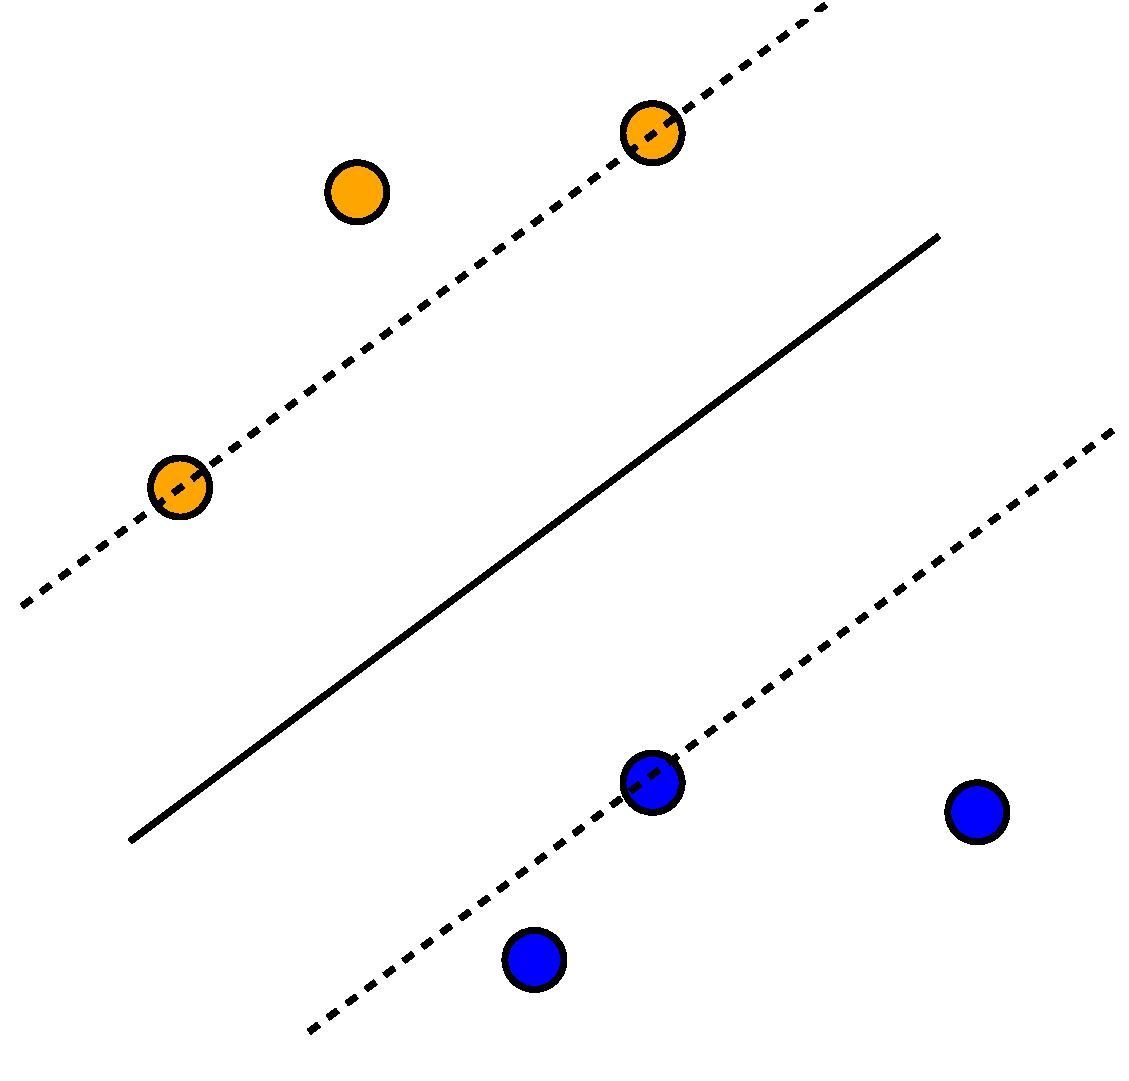
\includegraphics[width=0.3\columnwidth]{images/semi-supervised-advantage1}
B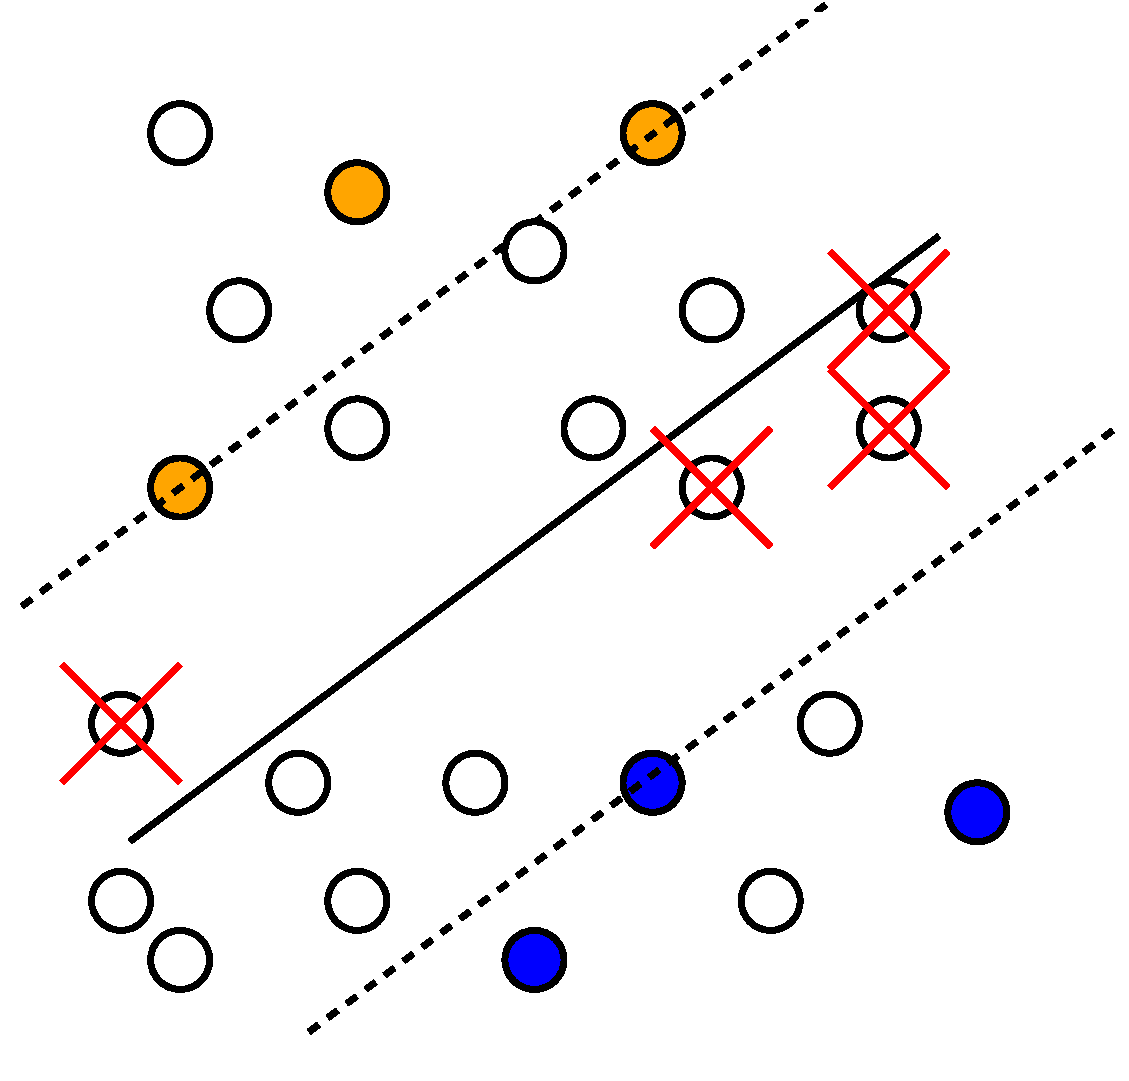
\includegraphics[width=0.3\columnwidth]{images/semi-supervised-advantage2}
C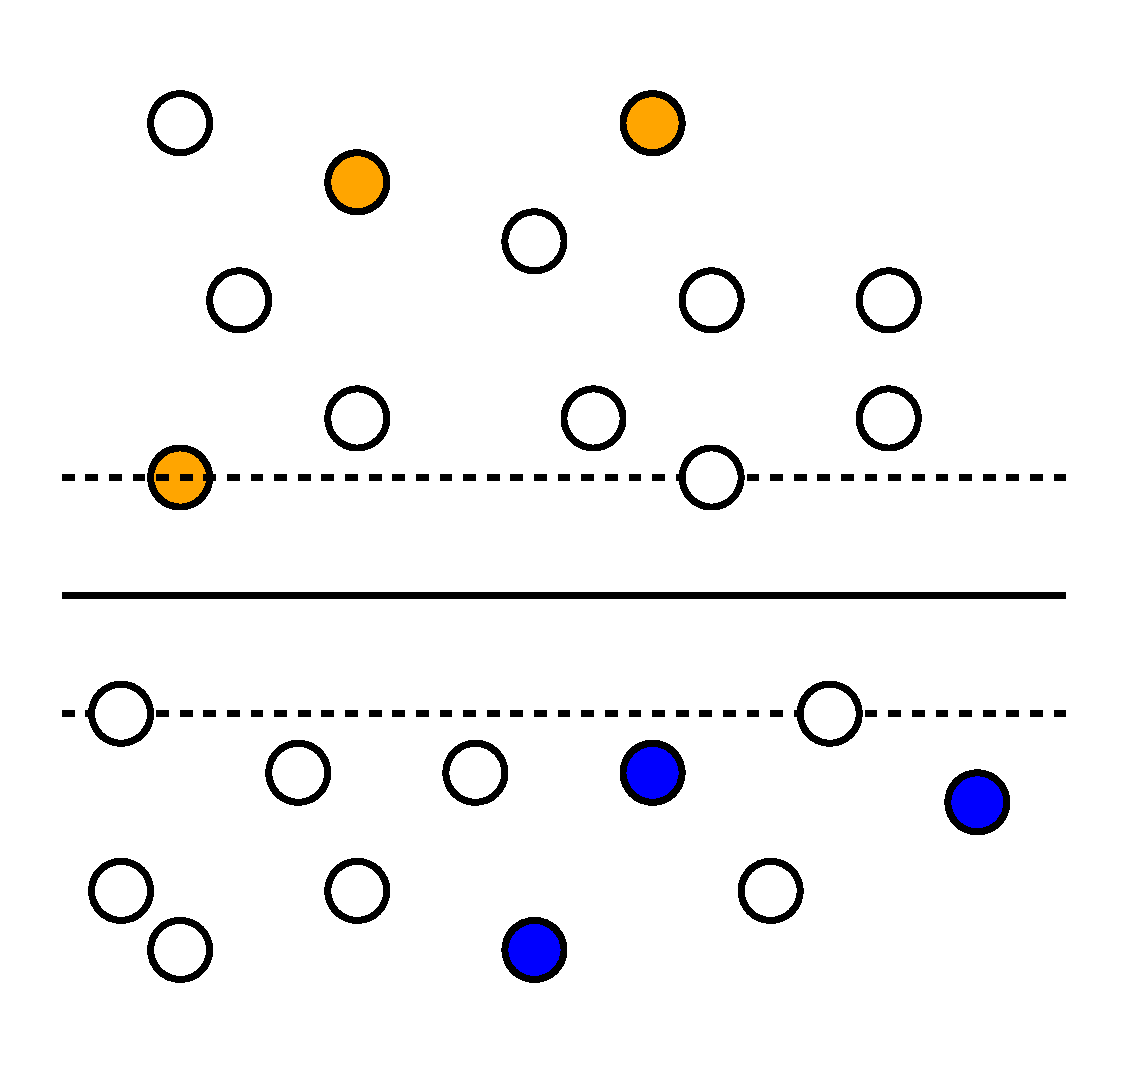
\includegraphics[width=0.3\columnwidth]{images/semi-supervised-advantage3}
\par\end{centering}
\caption[Illustration of semi-supervised learning in two dimensions.]{\label{fig:Illustration-of-semi-supervised-learning}Illustration
of semi-supervised learning in two dimensions. Each axis is a dimension.
Circles are samples; filled circles are labeled samples; unfilled
circles are unlabeled samples. The blue circles are samples with label
1, the orange circles are samples with label 2. A: Supervised SVM
learning produces a maximum-margin classifier. B: Supervised learning
ignores and probably mis-classifies some unlabeled samples (the red
crossed-out samples). C: Semi-supervised learning regards densities
of unlabeled samples and may give better results than supervised learning
on the labeled samples alone.}
\end{figure}

There are two types of semi-supervised learning: transductive and
inductive semi-supervised learning. The goal of transductive semi-supervised
learning\index{transductive semi-supervised learning} is to predict
the class labels of a pre-specified list of unlabeled input patterns,
while the goal of inductive\index{inductive semi-supervised learning}
semi-supervised learning is to find a universal rule mapping from
the space of input patterns to class labels, which could be applied
to classify unknown, future input patterns. In case unknown, future
input patterns are to be classified using transductive semi-supervised
machine learning, the whole model may have to be re-evaluated.

\subsubsection{Example Scenarios for Semi-supervised Learning}

An advantage of semi-supervised learning over supervised learning
is that it does not need labels for all input patterns, because labels
are often time-consuming or costly to acquire. For example, the Gene
Expression Omnibus data base (GEO) \cite{BarrettSoboleva2013} contains
41,379 expression data sets that were uploaded between Jan 1st, 2000,
and August 31st, 2013. Many of these are potentially usable as unlabeled
data sets in semi-supervised learning.

However in practice, many machine learning algorithms require samples
to be independently and identically distributed\index{independetly and identically distributed}
(iid\index{iid}). In an ideal world, GEO samples could be assumed
to be identically distributed within a data set. Unfortunately even
within the same GEO data set there often is systematic variation between
samples, called the \emph{batch-effect}\index{batch-effect}, caused,
for example, by different sample handling or conditions at measurement
time. Hence one either has to use samples from one data set only,
or, if one wants to use samples from different GEO data sets simultaneously,
correct for a possible batch-effect manually, or use an algorithm
that has some built-in mechanism to make such a correction.

One machine learning algorithm with such a built-in mechanism is\emph{
deep learning}\index{deep learning}, as employed in \emph{Deep Belief
Networks}\index{Deep Belief Network}\emph{ (DBNs}\index{DBN}\emph{)}
\cite{HintonTeh2006}. This machine-learning algorithm (which is unsupervised,
but can be used for supervised and semi-supervised learning) can learn
from images of objects or faces, where the objects or faces are in
different lighting conditions or are viewed from different angles
(\cite{HintonSalakhutdinov2006,KrizhevskyHinton2012,KarpathyFei-Fei2014}).
In this setting, the batch effect would be the lighting condition
or viewing angle. Such results seem to imply that DBNs are able to
abstract the images, which are given as vectors of pixels, into encodings
of relevant features and compute a classifier on these abstract features.
This can be seen as a form of batch-effect correction.

An extreme form of batch-effect correction is when all training data
are in batch 1 and all test data in batch 2. Are neural networks able
to handle such a situation? For example, suppose that batch 1 are
all face portraits (frontal view), batch 2 are half profile faces
(30 degree angle view) of \textendash{} not necessarily the same \textendash{}
people, and the task is to match faces seen from both viewing angles
to the same person. During training, semi-supervised learning would
have access to the unlabeled faces from both viewing angles, but all
the half profiles would be unlabeled. We are not aware of a study
of that setting using artificial neural networks, but a similar setting
was studied in cognitive psychology, where humans were the learners
\cite{BobakBate2015}. The participants of the study were asked to
match a given half profile to one out of 10 portraits, or indicate
that there is no matching face. The accuracy of average people was
81\%, while people who have extraordinary face recognition abilities,
so-called ``super-recognizers'', had 94\% accuracy. When there was
no matching face, average people correctly rejected the face in 65\%
of all cases, and super-recognizers did so in 92\%. For humans, the
unsupervised training would consist in seeing people's faces from
different angles during normal day-to-day activity. However, one could
argue that this training is unfair, because humans had access to the
label of many half profiles, since they often have seen a person's
portrait just moments before seeing the half profiles.

\subsection{Deep Learning}

Deep learning\index{deep learning} is a term used in artificial neural
networks with several hidden layers. The advantage of a deep network
over a network with just one hidden layer is that it can model a problem
more compactly using less hidden neurons in total, because it has
more than one intermediate computation step.

\emph{Autoencoders} and \emph{Deep Belief Networks}\index{Deep Belief Network}\emph{
}(\emph{DBNs}\index{DBN}) overcame the limitation of only a few hidden
layers \cite{BengioLarochelle2007,HintonTeh2006}. Here we give brief
overviews over both types of artificial neural network.

\paragraph{Autoencoder}

An autoencoder is a network with more than one hidden layer, whose
training is unsupervised and its objective is to reconstruct the input
in the output layer. An autoencoder starts as a three-layer network
composed of input layer, hidden layer, and output layer. This network
is trained using back-propagation. The middle hidden layer is then
copied and new hidden layer is inserted between both copies, forming
a five-layer-network. The newly added parameters of this network are
the same in number compared to a three-layer network, which can be
trained using back-propagation. Hence, training the five-layer-network
using back-propagation also works, and adding a new hidden layer in
the middle can be repeated.

\paragraph{Deep Belief Network}

Training a Deep Belief Network is separated into a pre-training phase
and a fine-tuning phase. The pre-training phase is unsupervised. It
starts with a network consisting of one input layer and a hidden layer.
This pair of  layers is called a \emph{Restricted Boltzmann Machine}\index{Restricted Boltzmann Machine}
(RBM\index{RBM}). There is an accompanying unsupervised training
procedure called \emph{contrastive divergence}\index{contrastive divergence}
which finds weights between these layers. After training the RBM,
hidden layers are iteratively added on top of the RBM, and the new
weights between layers are initialized and pre-trained using contrastive
divergence. While the pre-training phase is unsupervised, the fine-tuning
phase can be unsupervised as well as supervised. After training, the
multiple-hidden-layer-network forms a generative artificial neural
network called a Deep Belief Network.

\section{Overview of Own and Related Work}

We used autoencoders, Deep Belief Networks, and Transductive Support
Vector Machines on expression data to predict whether breast cancer
patients will show pathologic complete response to chemotherapy or
residual disease. The expression data are high-dimensional ($\approx22,000$
genes) and we use a relatively large data set ($\approx500$ patients).

\subsection{Motivations for Using Deep Belief Networks on Transcriptomic Data}

The motivations for using Deep Belief Networks on transcriptomic data
come from those networks' successes when used on image data. In the
hand-written digit classification and graphical object recognition
data sets on which the deep artificial neural networks were developed,
they are among the best-performing predictors.

\subsubsection{The ImageNet Large Scale Visual Recognition Challenge}

An example for the success of deep neural network is image classification
in the ImageNet Large Scale Visual Recognition Challenge \cite{RussakovskyFeiFei2015}.
It is a yearly contest, wherein participants are given around 1.2
million training images. Each training image is labeled with one of
$1,000$ possible object categories describing the main object appearing
in the image, for example ``trumpet'' or ``butterfly''. After
training an image classification algorithm, each contestant must compute
up to $5$ labels for each of $100,000$ test images. Each test image
has a single label, which is kept hidden by the contest organizer.
A test image is scored as correctly classified if the correct label
appears in the (up to $5$) labels submitted by the contestant. (Up
to 5 labels may be submitted because for example a street scene may
contain, besides the correct ``car'' label also street signs and
drivers.) Finally, the accuracy of a contestant is computed as the
average fraction of correctly classified test images.

There have been notable improvements in the accuracy of the winning
contestant, starting in 2012. In the last years, all top contestants
have moved to using deep neural networks. See table \ref{tab:ILSVRC-Test-set-accuracies}
for the winning contestants between 2010 and 2014. Significant differences
before and after 2012 are the usage of neural networks directly on
the image pixel data, and not using pre-computed image features in
a supervised learning algorithm like a Support Vector Machine.

\begin{table}
\begin{centering}
\begin{tabular}{|c|c|c|c|}
\hline 
Year & Winner & Accuracy & Technique\tabularnewline
\hline 
\hline 
2010 & NEC & 71.8\% & SIFT and LBP image features classified by SVM\tabularnewline
\hline 
2011 & XRCE & 74.2\% & image signatures classified by one-vs-all SVMs\tabularnewline
\hline 
2012 & SuperVision & 83.6\% & deep convolutional neural network\tabularnewline
\hline 
2013 & Clarifai & 88.3\% & deep convolutional neural networks averaged\tabularnewline
\hline 
2014 & GoogLeNet & 93.3\% & deep convolutional neural network\tabularnewline
\hline 
\end{tabular}
\par\end{centering}
\caption[Test set accuracies and techniques of winning contestants in the ImageNet
Large Scale Visual Recognition Challenge from 2010-2014.]{\label{tab:ILSVRC-Test-set-accuracies}Test set accuracies and techniques
of winning contestants in the ImageNet Large Scale Visual Recognition
Challenge from 2010-2014. Column ``Year'' is the year of the contest,
``Winner'' the team name of the winner of this year, ``Accuracy''
the test set accuracy of the winner's submission, and ``Technique''
a summary of the winner's algorithm technique. SVM, support vector
machine.}
\end{table}

\subsubsection{Highly Correlated Inputs}

We will now discuss similarities between image classification and
expression data classification.

Both underlying distributions \textendash{} of images and of expression
data \textendash{} have many correlated features. For images, adjacent
pixels often display the same object and have therefore correlated
values. In some face recognition tasks for example, the faces are
scaled and translated so that the centers of both eyes and mouth are
aligned in different faces. There will be highly correlated pixels
for areas of the image where the cheeks and lips usually are. If you
use the pixels of the whole image as input to the neural network,
the corresponding input nodes will be highly correlated as well.

For transcriptomic data, one almost always observes many correlated
genes. The correlations can be due to many genes being regulated by
the same transcription factor \cite{TornowMewes2003,KlebanovYakovlev2007}.

\subsubsection{Deep Belief Networks Find Correlated Nodes}

Deep Belief Networks can group correlated input nodes. The network
can do this by increasing the weights from the correlated group to
a single hidden node, and decreasing the weights from the group to
all other hidden nodes. The hidden node becomes the representative
of the correlated group of input nodes. This is a form of abstraction
and dimensionality reduction. The hidden node will only be active
if many of its highly-weighted input nodes are active and only few
of its negatively-weighted input nodes are active. Repeated application
of this principle of abstraction in deeper and deeper hidden layers
allows the Deep Belief Network to form more and more abstract representations
of its input.

In face recognition for example, an abstract representation might
have a single value for the size of the lips. In expression data,
a single node in an abstract representation might encode the activity
of a gene module.

\subsubsection{Transductive Support Vector Machine}

We compare the artificial neural network approach with another, older,
and established semi-supervised method, the Transductive Support Vector
Machine (TSVM) \cite{Joachims1999}. Despite the name, it supports
transductive as well as inductive learning. A standard Support Vector
Machine searches for a decision boundary such that the margin between
samples with differing labels is maximal (see figure \ref{fig:Illustration-of-semi-supervised-learning}).
The TSVM seeks a labeling of the unlabeled samples so that the decision
boundary has the maximal margin between all samples with differing
classes. 

\subsection{Previous Work: Gene Expression Inference With Deep Learning\label{subsec:Previous-Work:Gene-Expression-Inference-with-Deep-Learning}}

Very recently, \cite{ChenXie2015} published work on compressing expression
data into fewer dimensions on a large scale using deep learning. The
motivation for this work was that principal component analysis found
that $943$ ``landmark'' genes can capture about 80\% of the information
in the CMAP data set. This prompted the development of the ``L1000
Luminex bead technology'', which measures the expression of these
$943$ genes at a low cost, and computationally infers the remaining
$\approx21,000$ genes. \cite{ChenXie2015} worked on improving this
computational inference step.

Input data were all $\approx111,000$ genome-wide expression profiles
from the GEO database of Affymetrix microarrays, which were partitioned
into training, validation, and testing data sets. For each sample,
the same subset of $943$ landmark genes was chosen and $9,520$ other
genes were predicted from the landmark genes. This is different from
our work, because we classified breast cancer samples using gene expression
levels, while \cite{ChenXie2015} did regression of gene expression
levels using other gene expression levels.

\cite{ChenXie2015}'s artificial neural network architecture had between
$1$ and $3$ hidden layers with either $3,000$, $6,000$, or $9,000$
nodes. It had 943 input expression values (one for each landmark gene),
and a total of $9,520$ output expression values (one for each gene
to be predicted). In addition to the (non-linear) neural network,
they evaluated linear regression with no regularization, L1-, and
L2-regularization.

\cite{ChenXie2015} also evaluated k-Nearest Neighbor \index{k-Nearest Neighbor}(kNN\index{kNN}).
During training, they determined a number, $k$, of landmark genes
with expression value closest to each target gene $i$ (let's call
this set of genes $knn_{i}$) in the training data set. During testing,
they predicted the expression value of the target gene $i$ as the
average of the gene's $knn_{i}$ expression values in the testing
data set. The optimal $k$ (number of genes to average over) was chosen
based on a validation data set.

The input values were quantile normalized expression values between
4 and 15. The models were ranked according to the average prediction
errors over all 9,520 target genes.

k-Nearest Neighbor performed worst, with an average prediction error
of $0.5866$. Linear regression without regularization and with L2-regularization
both had an average prediction error of $0.3784$. Linear regression
with L1-regularization had an average prediction error of $0.3782$.
As the three linear regression models performed about equally well,
regularization did not improve linear regression. The neural network-based
average prediction errors were between $0.3421$ and $0.3204$, with
the network having $3$ hidden layers of size $9,000$ and $10\%$
dropout rate performing best. (\emph{Dropout }is a regularization
technique for neural networks, explained in section \ref{subsec:Dropout}.)
Because the input expression values were between $4$ and $15$, an
average prediction error of $0.3204$ implies an average error of
about $3\%$ on the GEO dataset.

In another dataset, \cite{ChenXie2015} again predicted $9,520$ genes
from the $943$ landmark genes, but used the GEO dataset for training,
the $1,000$ Genomes data for validation \cite{LappalainenPedro2013},
and GTEx data for testing \cite{ArdlieLek2015}. Learning in this
data set is harder since the training, validation, and testing data
sets are measured using different expression measurement technologies,
and therefore prone to the batch-effect. Nevertheless, the performance
ranking of the methods was the same, but worse than the data set without
batch-effect. KNN scored worst, with an average prediction error of
$0.6520$. Linear regression with L1-regularization had an average
prediction error of $0.5667$. Linear regression without regularization
and with L2-regularization both had an average prediction error of
$0.4702$. The artificial neural networks all scored consistently
better than KNN and linear regression, with the artificial neural
network with $2$ hidden layers of size $9,000$, and $25\%$ dropout
rate having the lowest prediction error of $0.4393$ (which is equivalent
to a relative error of $4\%$). On the validation data set, the average
prediction error was $0.7467$, which is a relative error of $6.8\%$.
This shows that artificial neural networks are capable of processing
input from multiple sources, with an acceptable gain in error. We
had a similar result, in section \ref{sec:Unsupervised-Reconstruction-of-Expression-Values}.
